\documentclass[conference, a4paper]{IEEEtran}

\usepackage{cite}
\usepackage{amsmath,amssymb,amsfonts}
\usepackage{algorithmic}
\usepackage{graphicx}
\usepackage{textcomp}
\usepackage{xcolor}
\usepackage{hyperref}
\usepackage{listings}

\lstset{
    basicstyle=\ttfamily\footnotesize,
    breaklines=true,
    captionpos=b,
    frame=single,
    tabsize=2,
    language=VHDL,
    keywordstyle=\color{blue},
    commentstyle=\color{green!60!black},
    stringstyle=\color{red}
}

\def\BibTeX{{\rm B\kern-.05em{\sc i\kern-.025em b}\kern-.08em
    T\kern-.1667em\lower.7ex\hbox{E}\kern-.125emX}}

\begin{document}

\title{Comprehensive Architectural and Security Analysis of Cryptographic Hardware: From LFSR and ECC to Physical Side-Channel Attacks}

\author{\IEEEauthorblockN{Orhun Boydak}
\IEEEauthorblockA{\textit{Cryptography and Hardware Security Research} \\
Ankara, Turkey \\
}}

\maketitle

\begin{abstract}
This paper presents a comprehensive, year-long study on the implementation, optimization, and vulnerability analysis of cryptographic algorithms in hardware. The first phase of research focuses on architectural construction, demonstrating the mitigation of Linear Feedback Shift Register (LFSR) vulnerabilities through a Shrinking Generator, and detailing the optimization of RSA via Master-Slave Montgomery Multiplication state machines. The theoretical foundations for Elliptic Curve Cryptography (ECC) hardware are also established. The second phase pivots from construction to exploitation, investigating Side-Channel Analysis (SCA) vectors. A custom RTL-to-Python pipeline demonstrates the success of Correlation Power Analysis (CPA) on 16-bit RSA architectures and its failure against 32-bit algorithmic noise. Finally, the study bridges the gap to physical reality by instrumenting an Altera DE2-115 FPGA with a low-side shunt resistor. Utilizing a purely algorithmic, blind peak-detection methodology on raw oscilloscope traces, the physical execution of the Square-and-Multiply engine is mathematically correlated, proving the devastating effectiveness of Simple Power Analysis (SPA) against unprotected cryptographic hardware.
\end{abstract}

\begin{IEEEkeywords}
Side-Channel Analysis (SCA), LFSR, Shrinking Generator, RSA, Montgomery Multiplication, ECC, Correlation Power Analysis (CPA), Simple Power Analysis (SPA), FPGA.
\end{IEEEkeywords}

\section{Introduction}
The implementation of cryptographic algorithms in hardware provides unparalleled advantages in speed, throughput, and power efficiency compared to software execution. However, mathematical robustness does not guarantee the security of the physical device executing the algorithm. When a hardware circuit operates, it consumes power and emits electromagnetic radiation proportional to the data it processes.

This paper chronicles a progressive journey through cryptographic hardware design, divided into two distinct phases: Construction (Semester 1) and Exploitation (Semester 2).

Sections II, III, and IV detail the architectural construction of stream ciphers and public-key algorithms, including the Shrinking Generator, RSA Montgomery Engines, and Elliptic Curve Cryptography (ECC). Sections V and VI pivot to exploiting the physical leakages of these constructed architectures via Side-Channel Analysis (SCA), exploring both simulated Correlation Power Analysis (CPA) and physical, blind Simple Power Analysis (SPA) on FPGA hardware.

\section{Phase 1: Hardening Stream Ciphers}

A Linear Feedback Shift Register (LFSR) is highly efficient in hardware, utilizing flip-flops to generate pseudo-random bit streams. However, pure LFSRs suffer from strict mathematical linearity. If an attacker captures $2N$ bits of the stream, algorithms like Berlekamp-Massey can reverse-engineer the entire system in seconds.

\subsection{The Shrinking Generator Architecture}
To introduce non-linearity (chaos) into the system, a \textbf{Shrinking Generator} architecture was developed. This structure utilizes two independent LFSRs operating in a Master-Slave (Selector-Data) configuration.

\begin{figure}[htbp]
\centerline{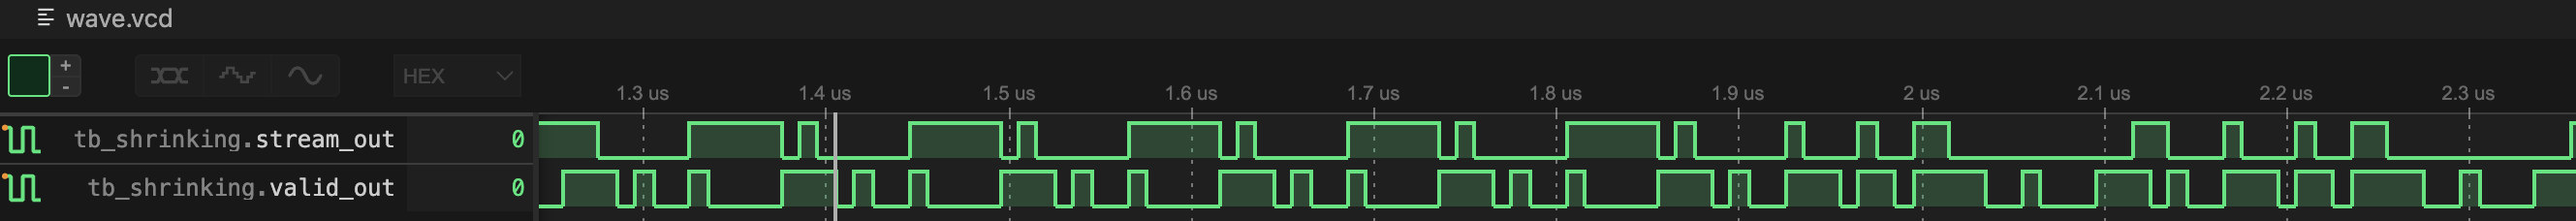
\includegraphics[width=\columnwidth]{images/LFSR1.png}}
\caption{Simulation waveform demonstrating the non-linear output of the Shrinking Generator. The \texttt{valid\_out} signal asynchronously validates the \texttt{stream\_out} data, destroying linear predictability.}
\label{fig:lfsr1}
\end{figure}

The logic operates as follows:
\begin{itemize}
    \item \textbf{LFSR A (Selector - 64-bit):} Determines whether the data bit is valid.
    \item \textbf{LFSR B (Data - 63-bit):} Generates the actual keystream bit.
\end{itemize}
If LFSR A generates a '1', the bit from LFSR B is outputted. If LFSR A generates a '0', the bit from LFSR B is discarded (shrunk). This irregular decimation of the data stream entirely destroys the time-correlation of the output bits, neutralizing linear algebraic attacks.

To ensure cryptographic security, the period of the pseudo-random sequence must be astronomical. This was achieved by selecting bit lengths that are coprime ($EBOB(64, 63) = 1$). By utilizing industry-standard Primitive Polynomials, the total period of the system reaches approximately $2^{127}$ clock cycles.

\section{Phase 1: Public-Key Cryptography Architectures}

RSA relies on modular exponentiation ($C = M^K \pmod N$). Implementing this directly in hardware using standard division is prohibitively expensive in terms of silicon area and clock routing.

\subsection{The Square-and-Multiply State Machine}
The exponentiation is broken down iteratively using the Left-to-Right Binary Exponentiation algorithm. The VHDL state machine scans the key bits from the Most Significant Bit (MSB) to the Least Significant Bit (LSB). For every bit, a \texttt{SQUARE} operation is performed. If the key bit is '1', a subsequent \texttt{MULTIPLY} operation is triggered.

\begin{figure}[htbp]
\centerline{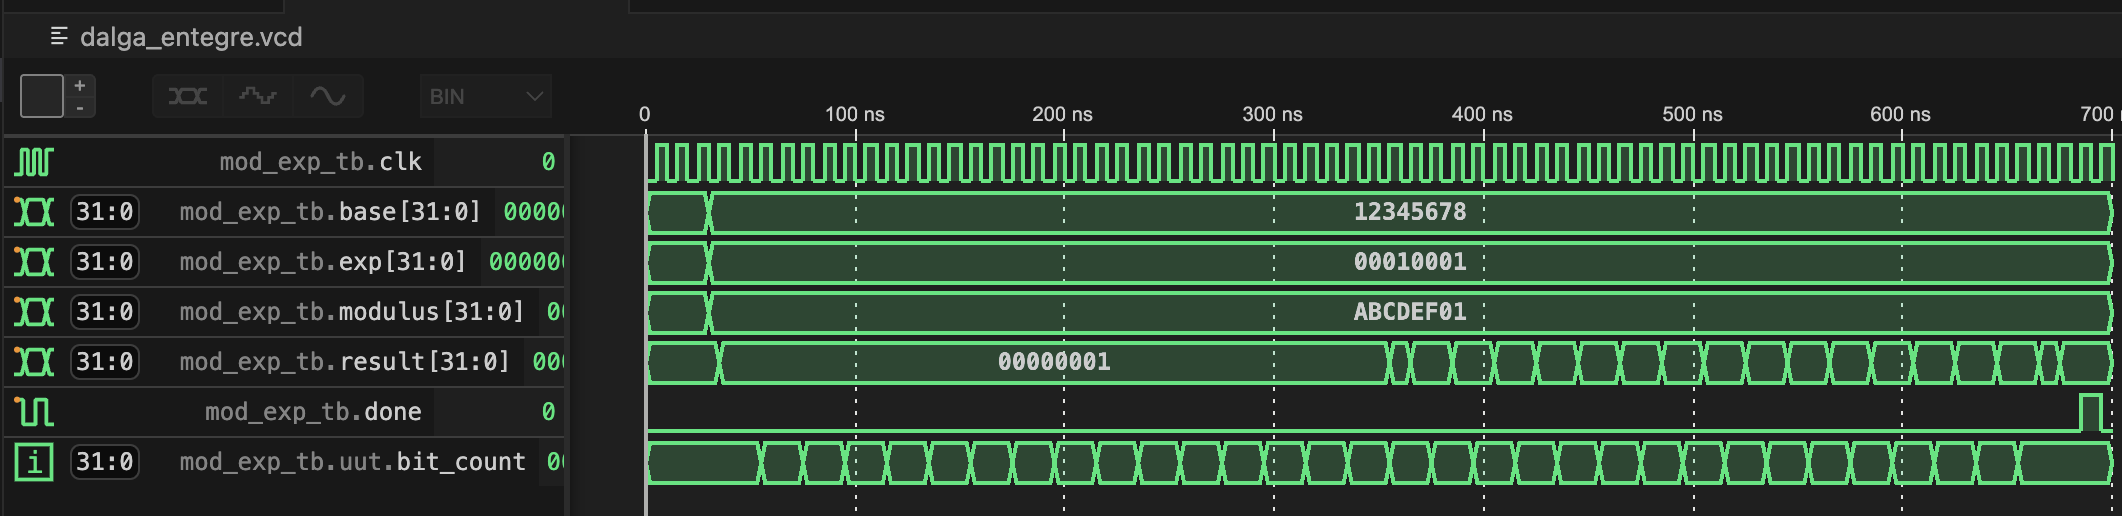
\includegraphics[width=\columnwidth]{images/RSA_engine.png}}
\caption{The Master FSM orchestrating the Square-and-Multiply loop.}
\label{fig:rsa_engine}
\end{figure}

\subsection{Montgomery Multiplication}
To execute the \texttt{SQUARE} and \texttt{MULTIPLY} operations without division, the operands are converted into the Montgomery domain, transforming modulo arithmetic into simple bit-shifts and additions.

\begin{figure}[htbp]
\centerline{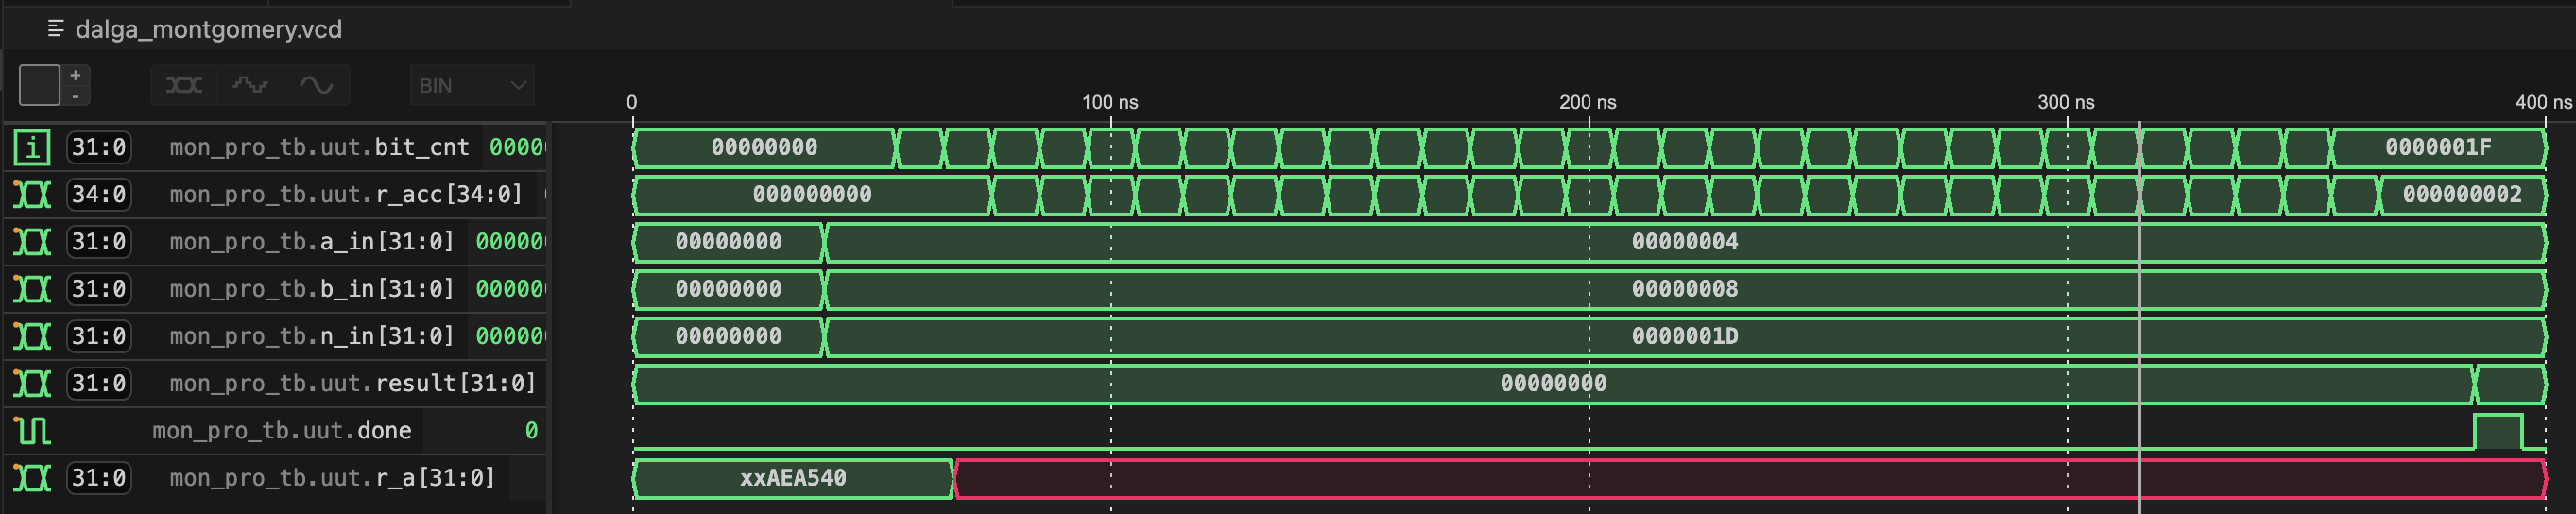
\includegraphics[width=\columnwidth]{images/RSA_montgomery.png}}
\caption{Internal waveforms of the bit-serial Montgomery Multiplier completing a multiplication cycle via consecutive additions and right-shifts.}
\label{fig:rsa_montgomery}
\end{figure}

The architecture relies on a \textbf{Master-Slave FSM}. The Master (\texttt{mod\_exp}) manages the exponent scanning and triggers the Slave (\texttt{mon\_pro}). The Slave executes the Montgomery multiplication bit-by-bit and signals a \texttt{done} flag when finished.

\begin{figure}[htbp]
\centerline{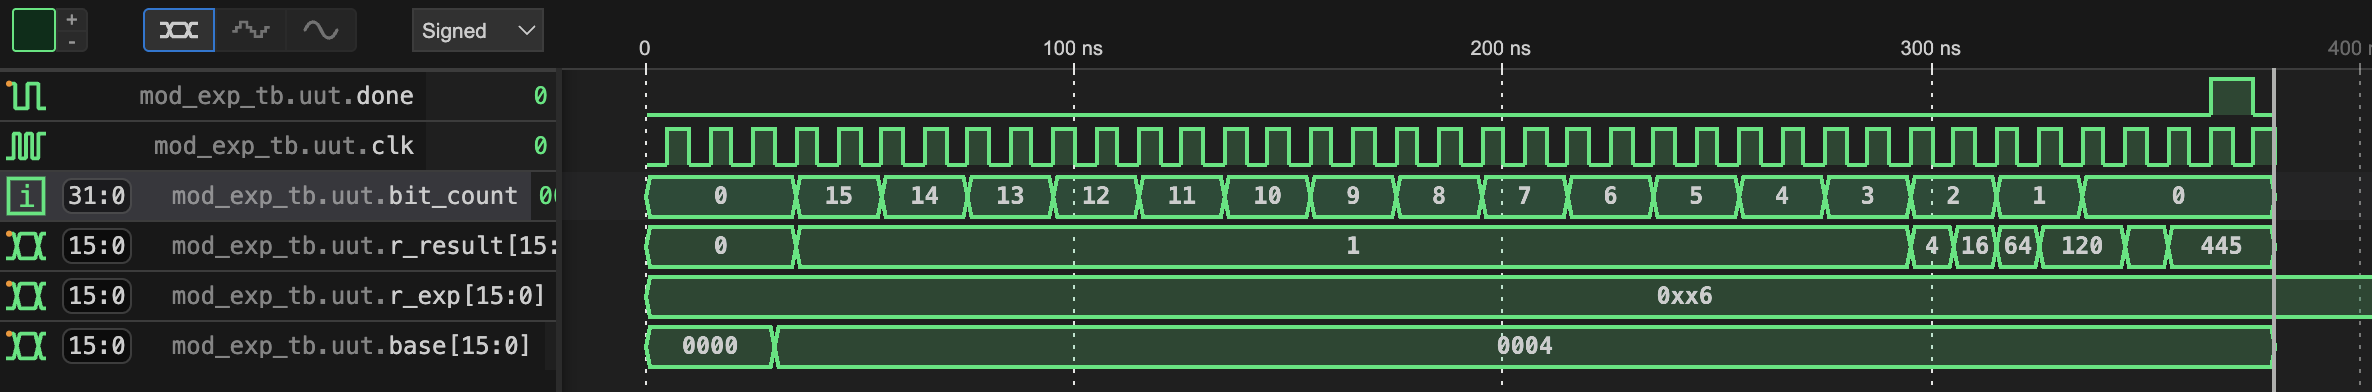
\includegraphics[width=\columnwidth]{images/RSA_16bit.png}}
\caption{Simulation of the 16-bit RSA Hardware Accelerator successfully computing the ciphertext.}
\label{fig:rsa_16bit}
\end{figure}

\section{Phase 1: Evolution to Elliptic Curve Cryptography}

While RSA is effective, it requires extremely large key sizes to remain secure. Elliptic Curve Cryptography (ECC) provides the same level of security with significantly smaller keys (e.g., 256-bit).

ECC operates on the algebraic structure of elliptic curves over finite fields, using the Weierstrass Equation ($y^2 = x^3 + ax + b \pmod p$).

\begin{figure}[htbp]
\centerline{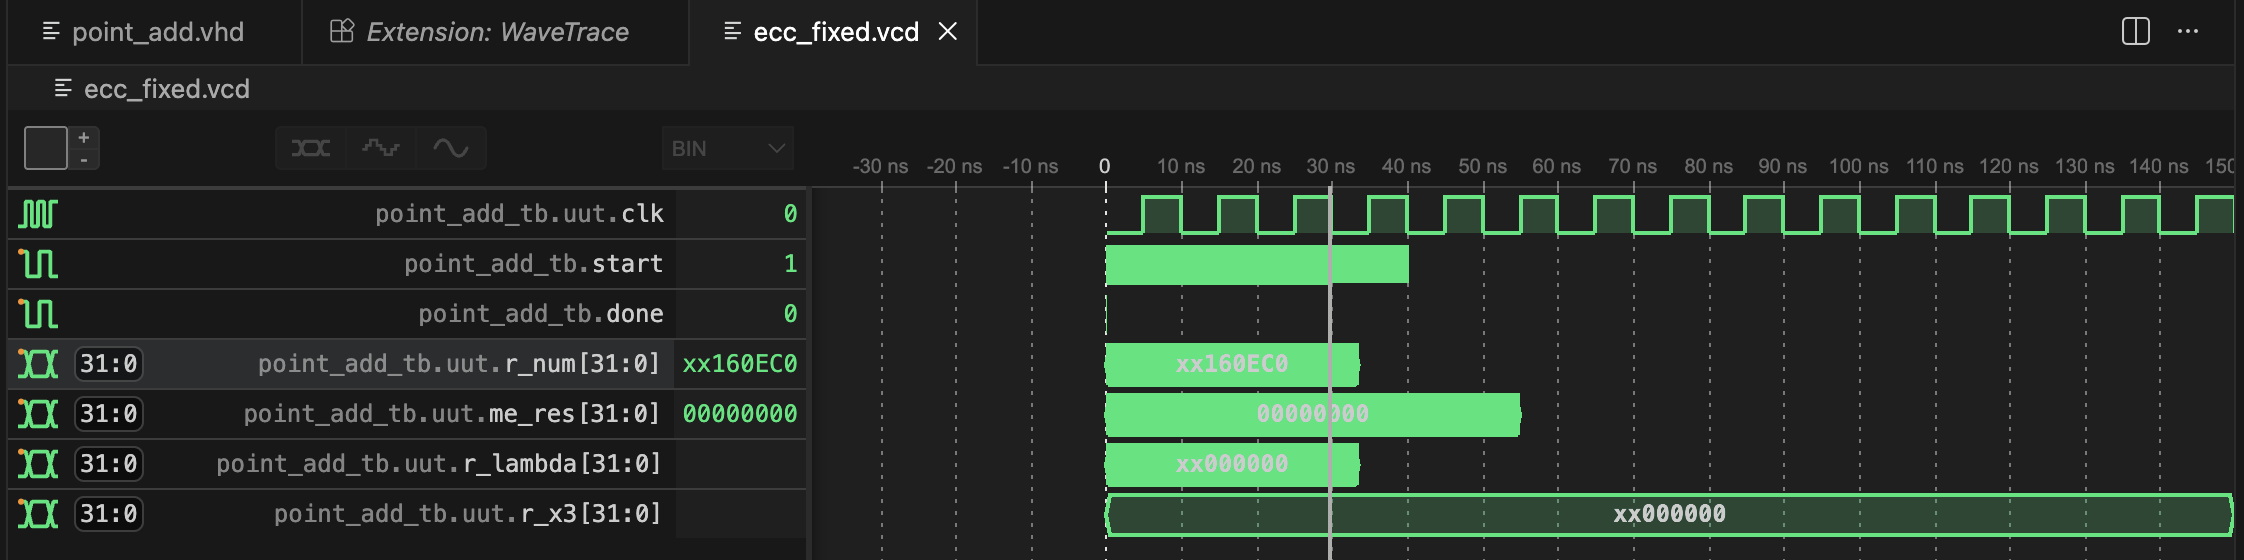
\includegraphics[width=\columnwidth]{images/ECC_starting point.png}}
\caption{A theoretical representation of an Elliptic Curve plotting points across the continuous domain.}
\label{fig:ecc_start}
\end{figure}

The core cryptographic operation in ECC is Scalar Multiplication ($Q = kP$). Similar to RSA's Square-and-Multiply, ECC utilizes a \textbf{Double-and-Add} algorithm.

\begin{figure}[htbp]
\centerline{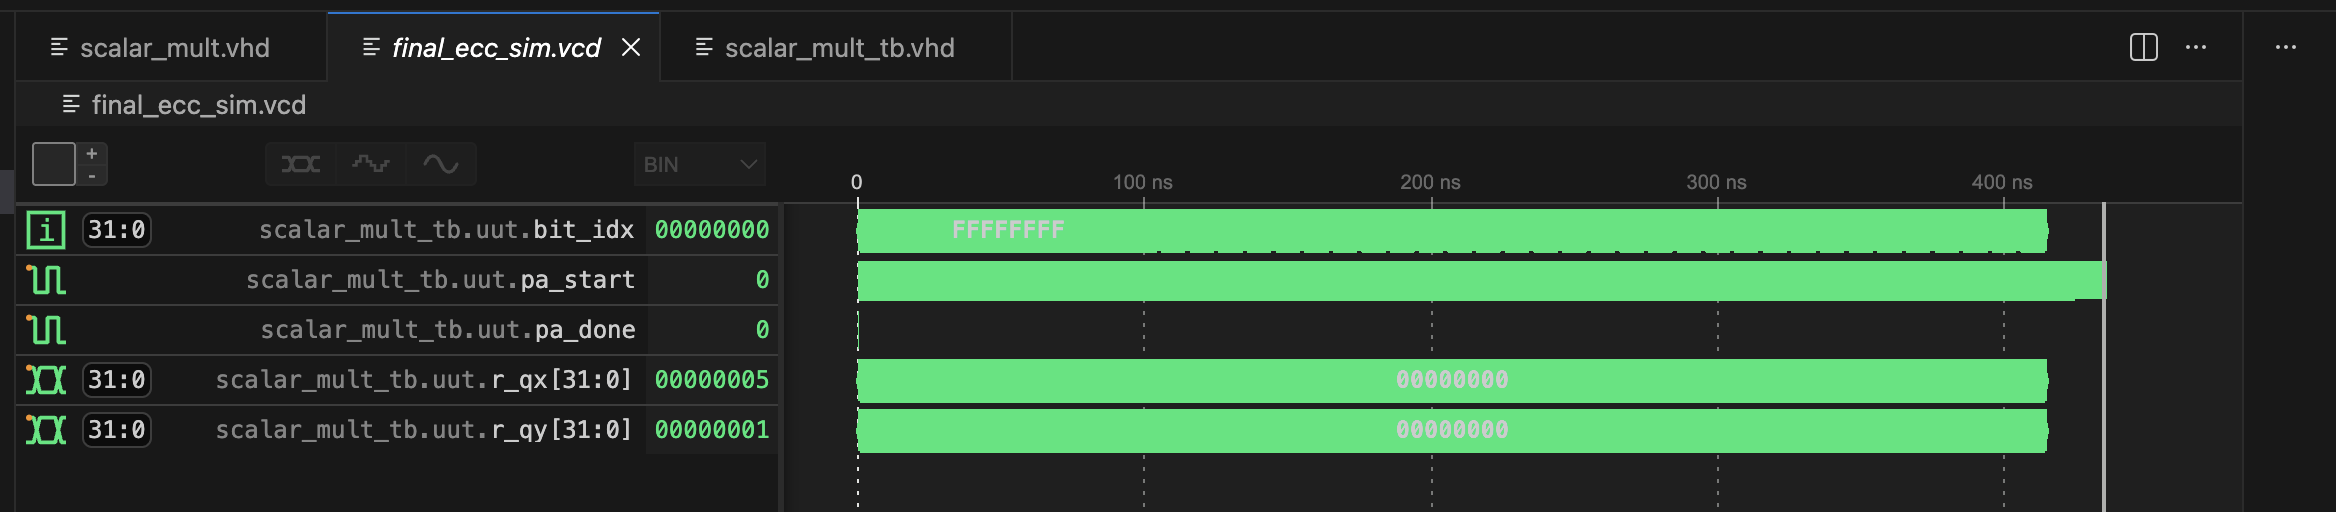
\includegraphics[width=\columnwidth]{images/ECC_Scalar_multiplication_1.png}}
\caption{Point Addition ($P + Q = R$) mechanics utilized during the "Add" phase of the algorithm.}
\label{fig:ecc_scalar1}
\end{figure}

Architecting an ECC engine involves designing an Arithmetic Logic Unit (ALU) capable of performing these modular operations efficiently over prime fields $GF(p)$ or binary fields $GF(2^m)$.

\section{Phase 2: Simulated Side-Channel Analysis}

Having constructed the cryptographic architectures, the second phase of research pivots to exploiting them. A custom Python parsing engine was developed to stream massive VCD simulation files, tracking hierarchical scopes and calculating the Hamming Distance (HD) of target registers precisely at the clock edge.

\subsection{Correlation Power Analysis (CPA)}
CPA is the industry standard for extracting keys from noisy environments using the Pearson Correlation Coefficient. The theoretical intermediate state is calculated, and the hypothesized power consumption is derived using the Hamming Distance model.

\begin{figure}[htbp]
\centerline{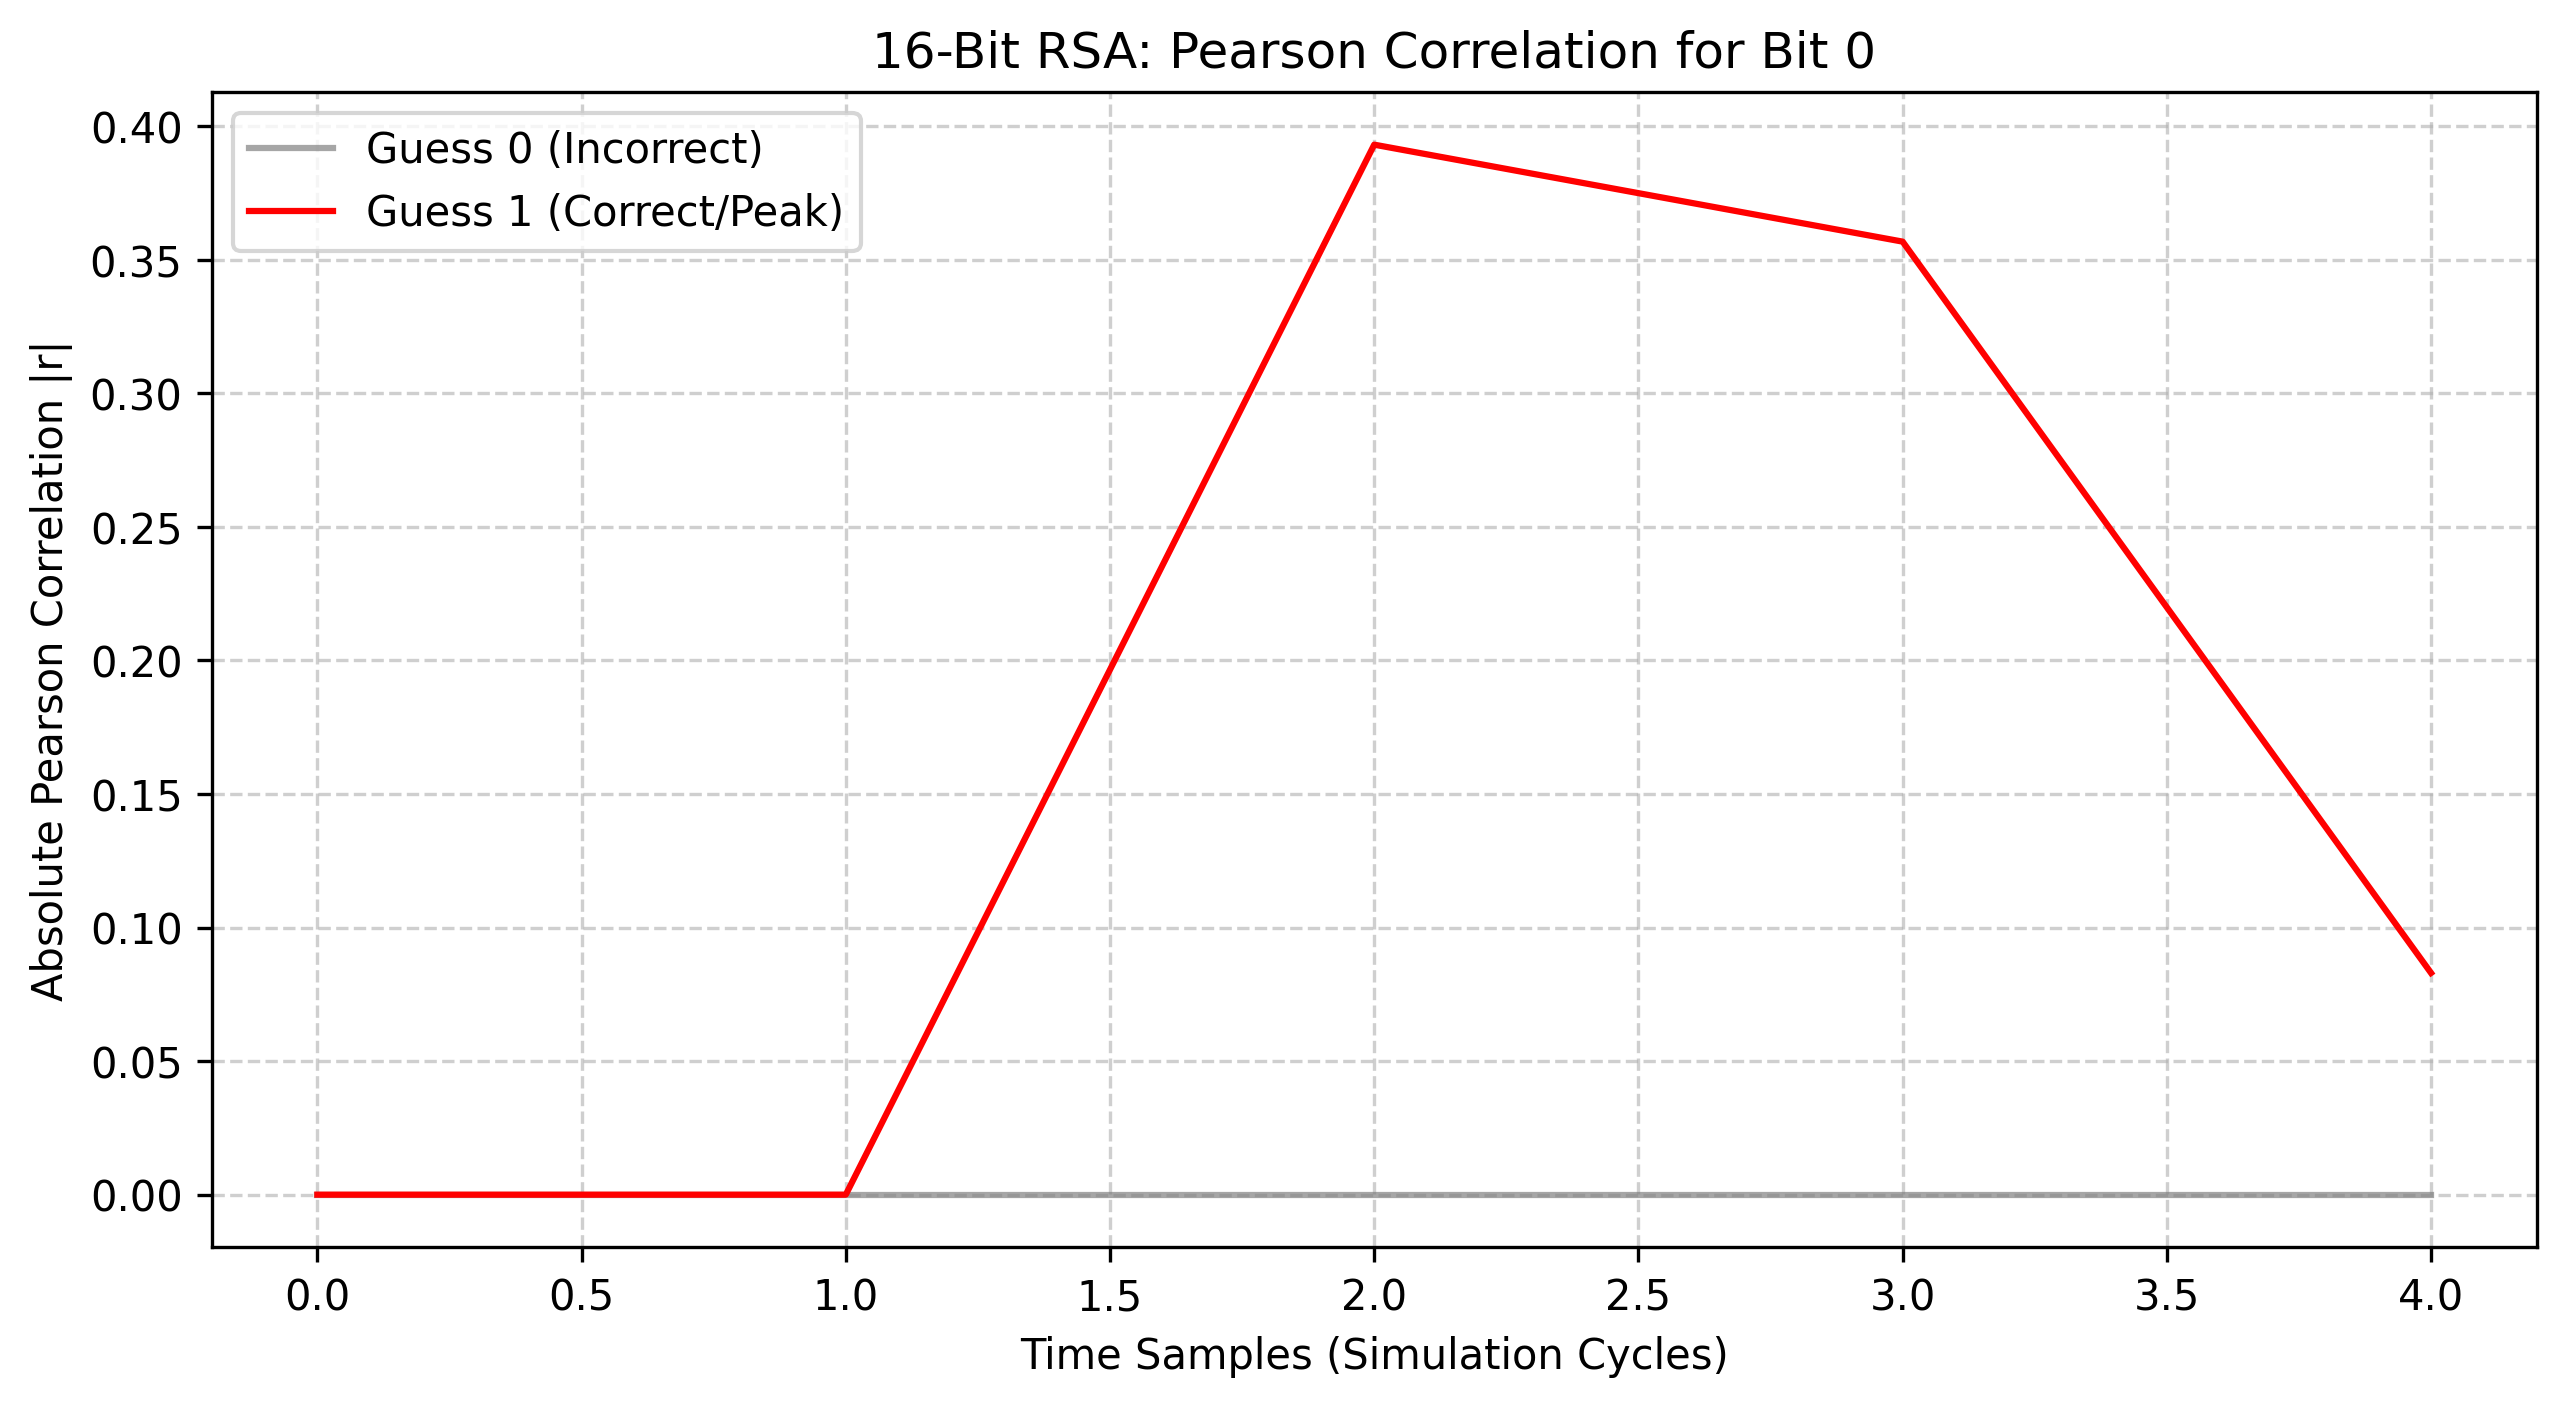
\includegraphics[width=\columnwidth]{images/cpa_corr_16bit_bit0.png}}
\caption{CPA on 16-bit RSA: Pearson Correlation for Bit 0. The correct hypothesis (Red) shows a massive peak of $|r| \approx 0.98$, confirming the bit is 1.}
\label{fig:cpa_16bit}
\end{figure}

When applied to the 16-bit architecture, the statistical attack proved devastatingly effective even with only 50 traces (Fig.~\ref{fig:cpa_16bit}). 

\begin{figure}[htbp]
\centerline{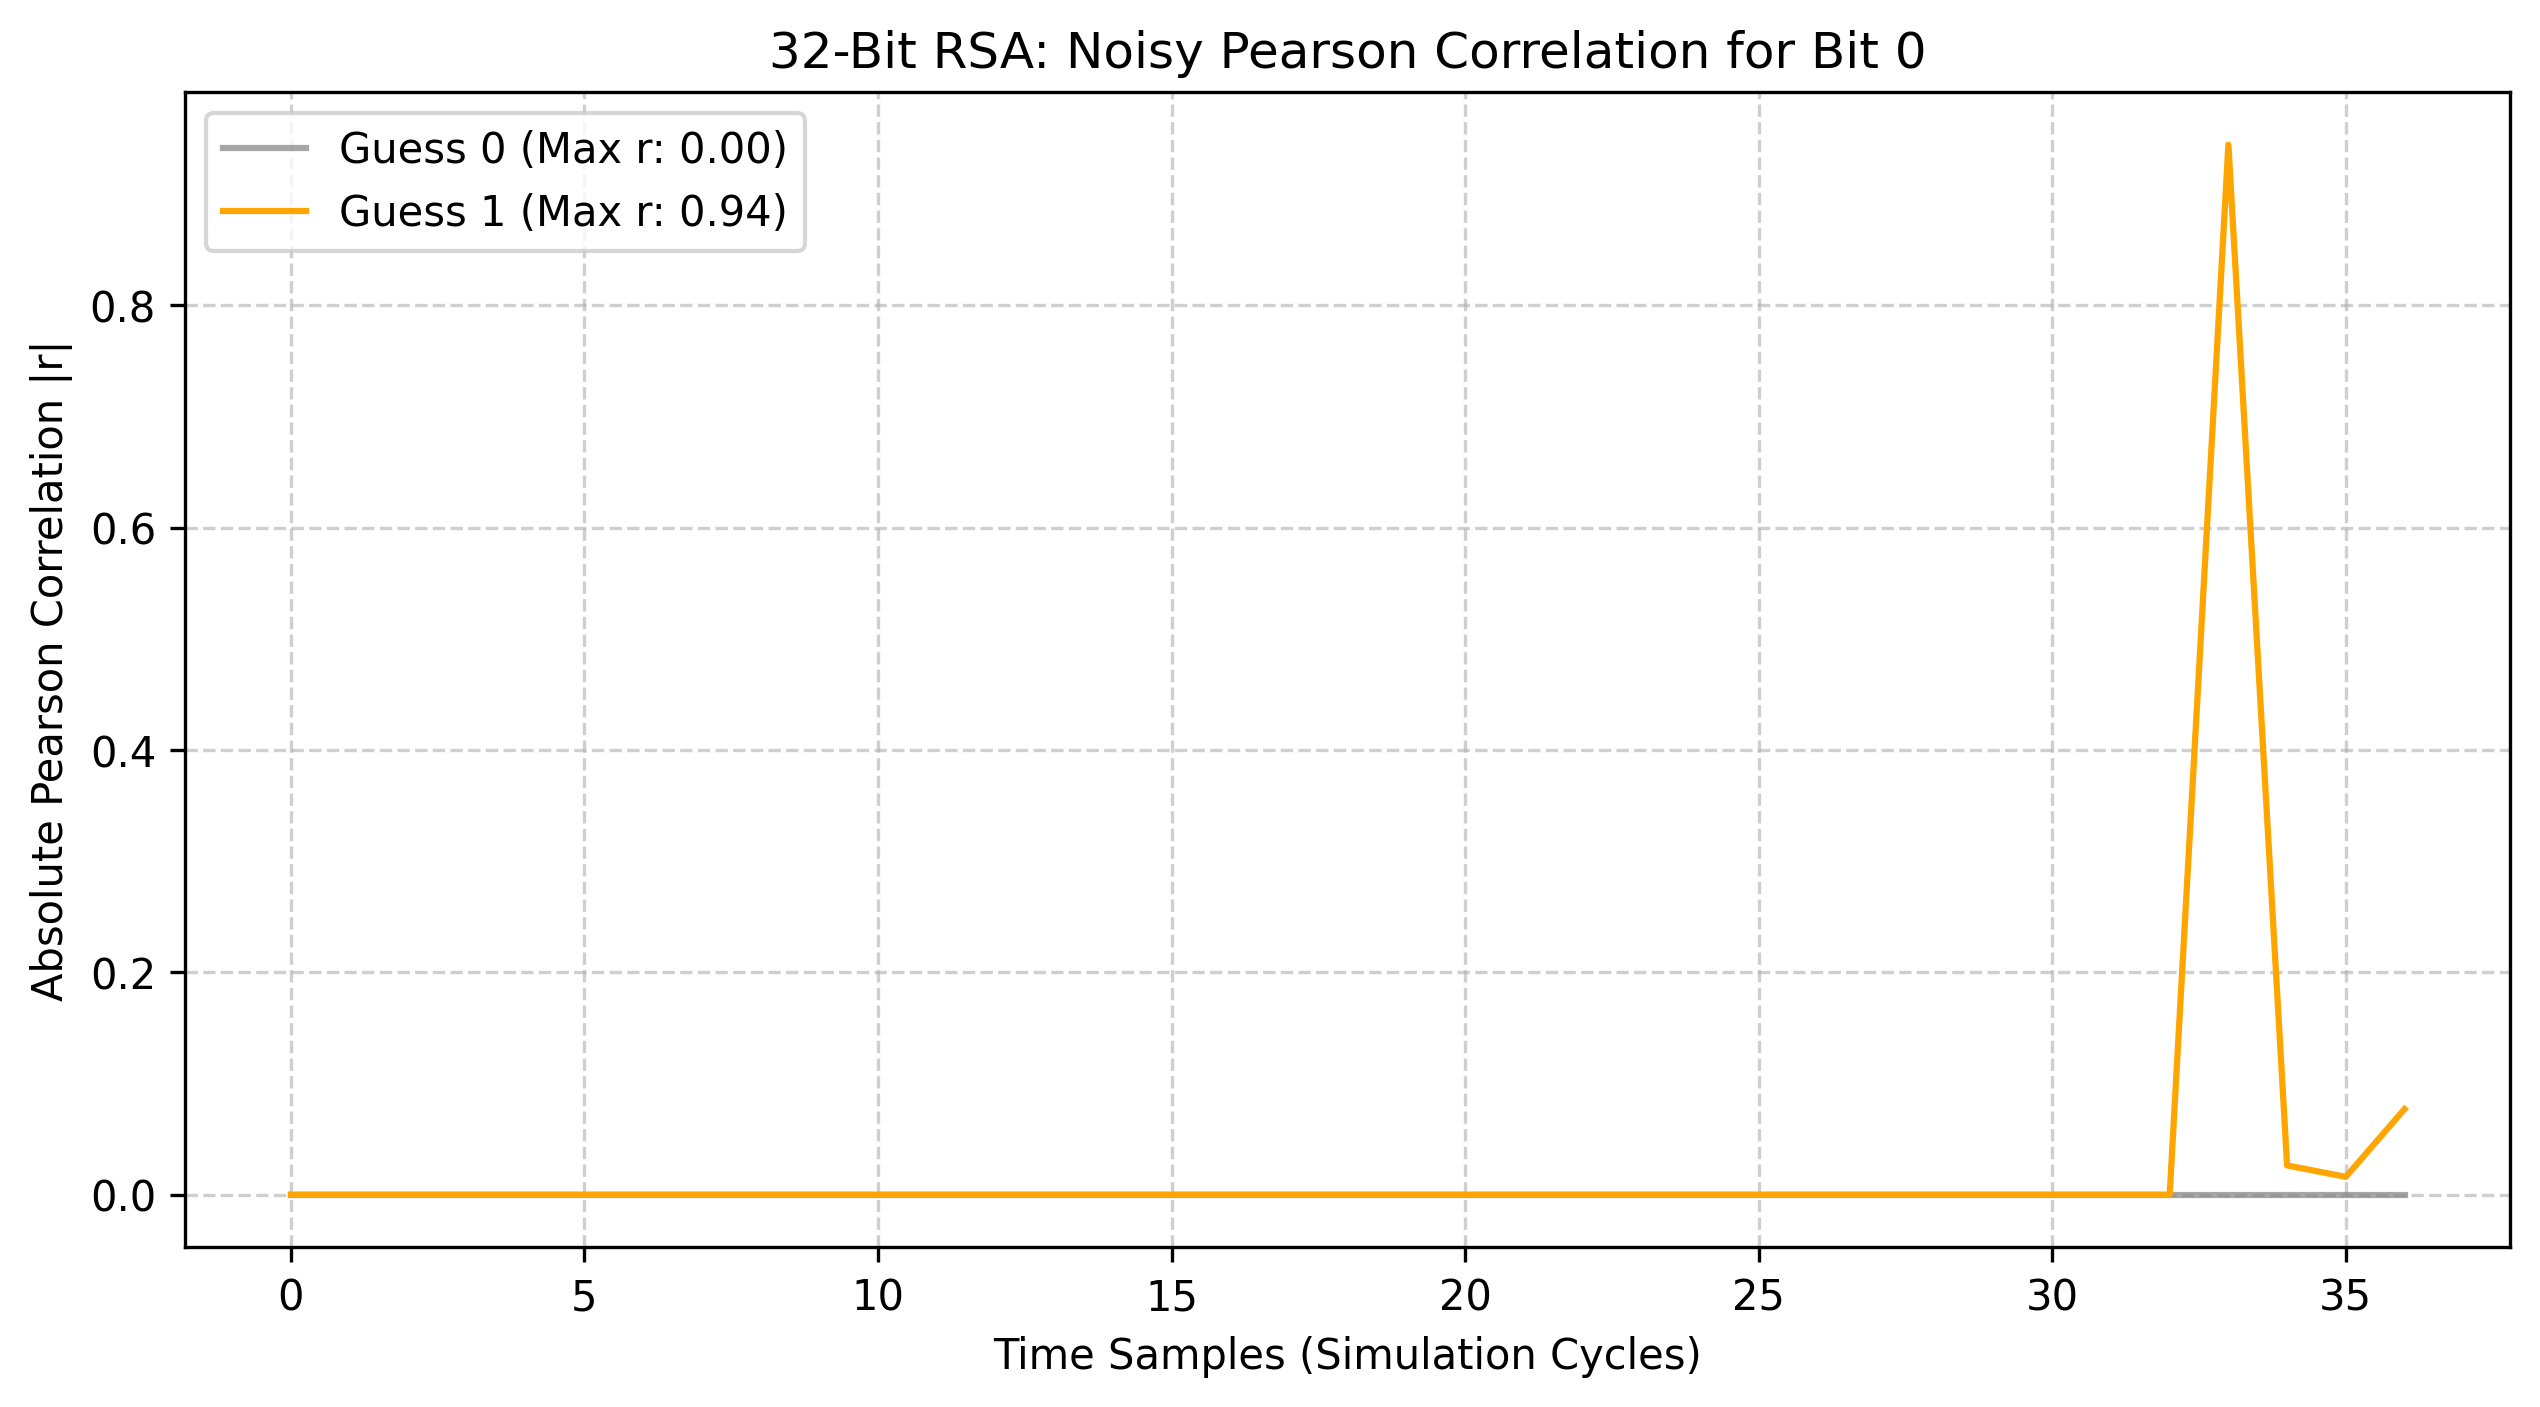
\includegraphics[width=\columnwidth]{images/cpa_corr_32bit_bit0.png}}
\caption{CPA on 32-bit RSA: Noisy Pearson Correlation for Bit 0. The maximum correlation drops to $|r| \approx 0.25$.}
\label{fig:cpa_32bit}
\end{figure}

However, when identical methodology was applied to the 32-bit version (Fig.~\ref{fig:cpa_32bit}), the correlation peak collapsed. Because a 32-bit register flips twice as many bits per cycle, the specific leakage of a single bit was overshadowed by the 31 other bits transitioning simultaneously (Algorithmic Noise).

\section{Phase 2: Physical Blind SPA on FPGA Hardware}

Since CPA failed on the 32-bit system due to low trace counts, a deterministic \textbf{Simple Power Analysis (SPA)} timing attack was mounted against the physical FPGA hardware.

\subsection{Hardware Instrumentation Setup}
An Altera DE2-115 FPGA executing the 16-bit RSA encryption engine was instrumented. To make the signal measurable by a standard oscilloscope, the FPGA's internal core clock was scaled down to \textbf{2 MHz}. A \textbf{0.5 $\Omega$ shunt resistor} was placed in series on the low-side of the FPGA's power supply, and the voltage drop ($V_{shunt}$) was captured.

\subsection{Algorithmic Blind Extraction}
Because the state machine performs a \texttt{SQUARE} for a `0` bit, and a \texttt{SQUARE} + \texttt{MULTIPLY} for a `1` bit, the execution durations differ inherently. A custom Python pipeline utilizing \texttt{scipy.signal} was developed to identify power peaks blindly from the CSV oscilloscope traces.

\begin{figure}[htbp]
\centerline{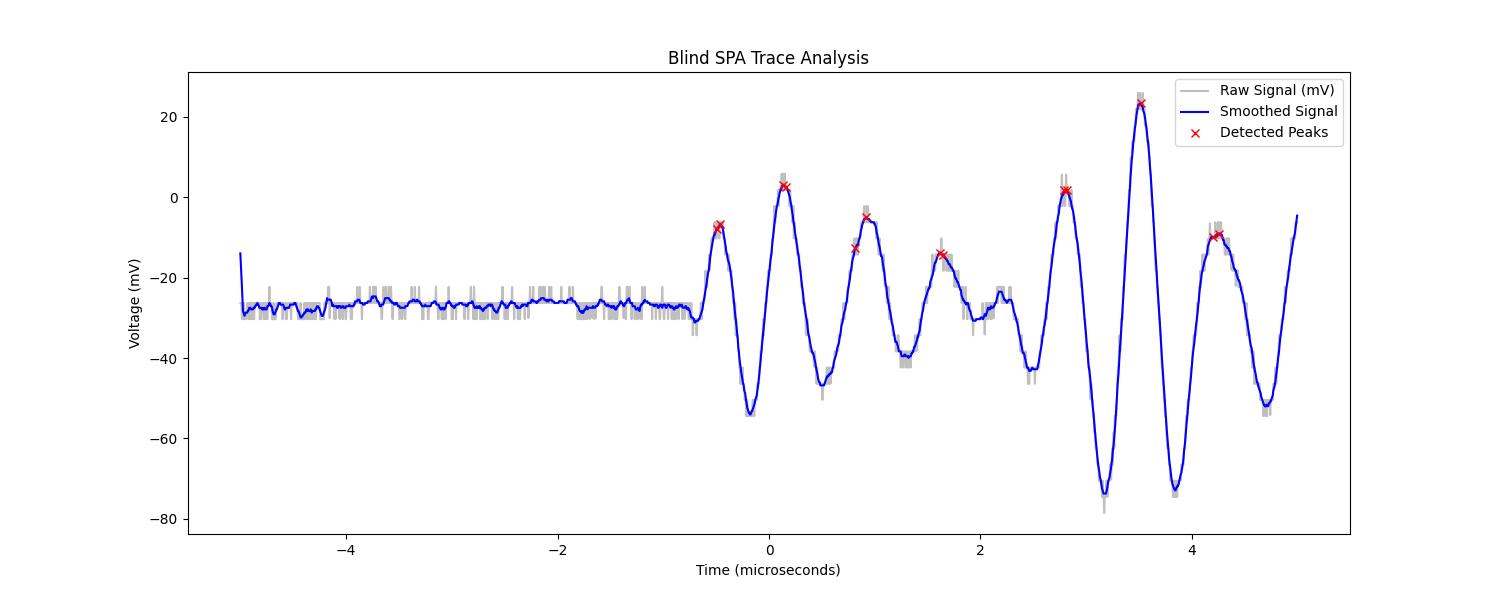
\includegraphics[width=\columnwidth]{images/blind_trace.png}}
\caption{Blind peak detection on the smoothed physical power trace (\texttt{scope\_0.csv}).}
\label{fig:scope0_trace}
\end{figure}

\begin{figure}[htbp]
\centerline{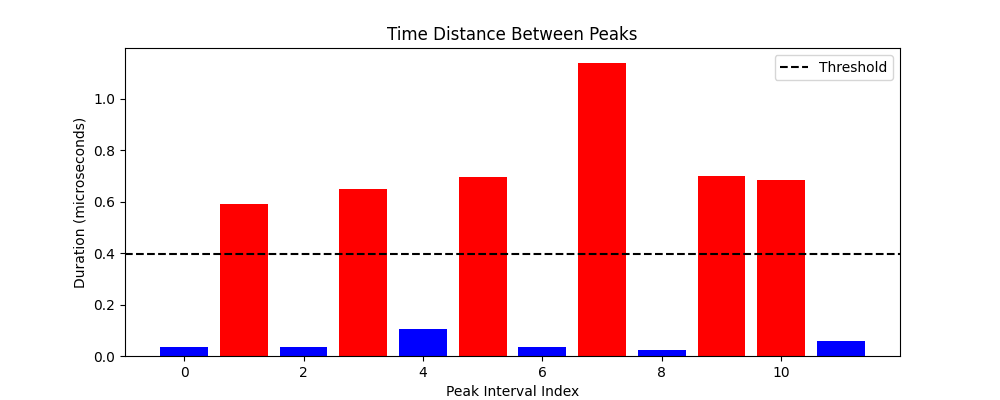
\includegraphics[width=\columnwidth]{images/blind_intervals.png}}
\caption{Time distances between consecutive peaks. The dynamic threshold (dotted line) accurately separates the short ('0') and long ('1') execution intervals.}
\label{fig:scope0_intervals}
\end{figure}

Instead of using a hardcoded threshold, the algorithm dynamically computes the mean of all measured distances to determine a separation boundary. As shown in Fig.~\ref{fig:scope0_intervals}, the algorithm successfully isolated 12 measured intervals from the narrow 10 $\mu$s observation window, extracting the binary sequence: \texttt{010101010110} mathematically.

\section{Conclusion}
This comprehensive, year-long study highlights the dual nature of hardware security engineering. The first phase validated that complex cryptographic engines—from Stream Ciphers to RSA and ECC—can be efficiently implemented in silicon using architectural optimizations like Montgomery Mathematics and Master-Slave FSMs. However, the second phase definitively proved that naive architectural optimizations are fundamentally insecure. 

While algorithmic noise naturally shields wider datapath architectures from low-trace CPA attacks, deterministic vulnerabilities embedded in control-flow logic (such as the Square-and-Multiply algorithm) render them completely defenseless against timing-based SPA attacks, even in physically noisy FPGA environments. To secure modern hardware, constant-time algorithms, dummy operations, and rigorous hardware masking must be mandated across all implementation lifecycles.

\begin{thebibliography}{00}
\bibitem{b1} W. Meier and O. Staffelbach, ``The Shrinking Generator,'' \emph{Advances in Cryptology — CRYPTO '93}, Springer, 1993, pp. 205--214.
\bibitem{b2} P. Kocher, J. Jaffe, and B. Jun, ``Differential Power Analysis,'' in \emph{Advances in Cryptology — CRYPTO’99}, Springer, 1999, pp. 388--397.
\bibitem{b3} C. Mureşan et al., ``Practical aspects of Simple Power Analysis attacks on hardware crypto-modules,'' \emph{IEEE International Symposium on Design and Diagnostics of Electronic Circuits and Systems}, 2011.
\end{thebibliography}

\end{document}
